\section{Approach}

We first present stress test operators which are used to create stress 
test cases for measuring model fragility,
%We first describe stress test operators for evaluating robustness in models. 
%, and adopt a subset of them as proxy test for short circuits. 
then propose two novel operations to augment training data to 
%reverse the short circuit problem and 
reduce short circuits in models.

\subsection{Stress Test Operators}
 \label{sec:stressop}
%The typical approach for detecting and 
%evaluating model fragility is to construct 
%out-of-distribution stress tests 
%in addition to the original in-distribution 
%test set and observe model 
%performance on these stress tests.

%In this paper, we consider the operators for constructing stress test listed in \tabref{table:proxyop}. 
%The operators were mentioned in previous literature\cite{checklist2020acl}. 
%%others are proposed here~(marked with *). 
%Each operator creates a stress test instance corresponding to a specific MCQ by keeping the right choice and 
%generating a new \textbf{wrong} choice. 

To evaluate the extent of model short circuits,  
we create these stress test cases using the operators
in \tabref{table:proxyop}. 
%Following previous research~\cite{checklist2020acl}, 
%we test the effectiveness of different data augmentation
%methods by looking at the robustness of models against
%different stress tests.
Most of the operators
have been proposed previously~\cite{checklist2020acl}, 
except for PR and PI, which
are newly introduced in this work.
We create a stress test instance from a specific MCQ by 
keeping the right choice and
creating a \textbf{wrong} choice by applying one of the
stress operators to the original right choice. This new
wrong choice is \textit{grammatically correct}
but \textit{logically incorrect} under the particular context. 
%Different operators generate different but sufficient number of cases 
%as shown in \tabref{tab:cases}. 
Besides, the new wrong choice contains the same content as the right choice 
except for the tested feature. 
These stress test cases with similar choices can evaluate 
%not only the general model robustness, but also
whether models 
%are exploiting spurious features in the choices 
%rather than 
are considering the connection between the premise and choices,
or in other words ``short-circuiting.'' 
For example, if a model 
doesn't comprehend the consistency of the 
NER name ``Mary'' in \tabref{tab:cases} which has
been mentioned in both the premise context and the right choice,  
then the model can be easily confused by a similar wrong choice. 
%for not considering the relation between the context and choices. 
\begin{table}[th!]
        \centering
        \scriptsize
        \begin{tabular}{l|l}
                \toprule
                \textbf{Oper.} &\textbf{Description and Example}\\
                \hline
                \multirow{3}{*}{Neg+} & Add negation (r$\rightarrow$w) \\
                & Input: \textit{They called the police to come to my house. \checksymbol} \\
                & Output: \textit{They {\textbf{{didn't}}} call the police to come to my house. \crosssymbol} \\
                \hline
                \multirow{3}{*}{Neg-} &Remove negation (r$\rightarrow$w) \\
                & Input: \textit{Ben {\textbf{never}} starts working out. \checksymbol} \\
                & Output: \textit{Ben starts working out. \crosssymbol}\\
                \hline

                \multirow{3}{*}{NER} &Randomly replace person names (r$\rightarrow$w)\\
                 & Input: \textit{A big wave knocked {\textbf{ Mary}} down. \checksymbol} \\
                & Output: \textit{A big wave knocked {\textbf{ Kia}} down. \crosssymbol} \\
                \hline
                \multirow{3}{*}{PR} & Switch pronoun by gender or quantity (r$\rightarrow$w)\\
        &Input: \textit{{\textbf{ She}} had a great time.\checksymbol} \\
        &Output: \textit{{\textbf{ He}} had a great time. \crosssymbol} \\
                \hline
                \multirow{3}{*}{PI} &Instantiate pronoun by random person (r$\rightarrow$w) \\
        &Input: \textit{{\textbf{ They}} gave Tom a new latte with less ice. \checksymbol}\\
        &Output: \textit{{\textbf{ Nathanael}} gave Tom a new latte with less ice. \crosssymbol}\\
        \hline
        \multirow{3}{*}{Voice} &Swap subject and object (r$\rightarrow$w) \\
        & Input: \textit{{\textbf{Kara}} asked {\textbf{the neighbors}}  not to litter in their yard. \checksymbol} \\
        & Output: \textit{{\textbf{the neighbors}} asked  {\textbf{Kara}}  not to litter in their yard. \crosssymbol}\\
%               %\hline
                %\multirow{3}{*}{Adv*} &Add adverbs for emphasis (w$\rightarrow$w)\\
                %&Input: \textit{The ocean was as calm as a bathtub .\crosssymbol} \\
                %&Output: \textit{{\textbf{ In fact}} the ocean was as calm as a bathtub .\crosssymbol} \\
  %:ew              \hline
              % \multirow{3}{*}{CO*} & Crossover: Swap the true choices between two questions (r$\rightarrow$w)\\ 
        %&Input: \textit{\textbf{olive}Josh got sick . \checksymbol} \\
        %&Output: \textit{\textbf{olive}{She had a great time .\crosssymbol}}  \\
%\hline
 %               \multirow{3}{*}{Syn} &Replace adj/adv with synonym (w$\rightarrow$w) \\
 %               &Input: \textit{Dawn felt {\textbf{ happy}} about getting away with it . \crosssymbol} \\
 %               &Output: \textit{Dawn felt {\textbf{ glad}} about getting away with it . \crosssymbol} \\
              % \multirow{3}{*}{MT*} & Mutate: Swap two consecutive words (r/w$\rightarrow$w) \\
        %       & Input: \textit{Deb said yes {\textbf{olive} to} {\textbf{olive} Tim} 's marriage proposal. \crosssymbol} \\
        %       & Output: \textit{Deb said yes {\textbf{olive} Tim} {\textbf{olive} to} 's marriage proposal .\crosssymbol} \\
        %       & Input: \textit{Josh {\textbf{olive}got sick}. \checksymbol} \\
        %       & Output: \textit{Josh {\textbf{olive} sick got}. \crosssymbol} \\
          %     \hline

                \bottomrule
        \end{tabular}
        \caption{Stress test operators considered in this paper.
The first line in each cell describes the operation, and the remaining lines in
the cell give examples of how the operators work.
r$\rightarrow$w indicates the operator turns a right choice into a wrong choice.}
%while
%w$\rightarrow$w indicates the operator turns a wrong choice into another wrong choice.}
        \label{table:proxyop}
\end{table}




\subsection{Improving Model Robustness by Data Augmentation}
\label{sec:aug}
%\KZ{I think this paragraph is kind of repeating the intro.}
%If a model is shown to be fragile by the stress tests, 
%its performance may decline, especially when applied to out-of-distribution test data.
%We make an assumption that these models are 
%limited by dataset and learned short circuits to make decision. 
%To make models more robust, 
To decrease short circuits in models, 
one natural thought is to generate more challenging training data that 
forces the models to focus on the relationship between the premise and choices.
A straight forward way to do this is to modify existing training data so that the 
right and wrong choices become similar to each other. For example, we could modify the 
right choice in an MCQ by
changing the named entity in it into another arbitrarily named entity and thus create a new
wrong choice that shares most of the features with the right choice.
But such an approach has two challenges: i) the modification operations are typically restricted to
a \textit{particular linguistic feature}, and hence it is hard to create data with good 
coverage of diverse
linguistic features; and ii) because some of the linguistic features may be sparse in the 
training data, the number of additional questions generated using these features may be very limited,
which means the data augmentation doesn't scale.
%But in reality, most of these operators are not scalable and 
%cannot generate enough data for training, e.g., \textit{NER} requires the presence of 
%named entities in the choices.
%Meanwhile, these stress test operators are fine-grained operations on specific features. 
%For example,  pronoun feature ``she'' may always co-occur with label ``right'', then we can balance this feature 
%in the training data.
%%\KZ{Can u explain a little what u mean by ``fine-grained'' operations on specific features, 
%%like some examples?}
%However, it's hard to enumerate all the possible features for training, not to mention 
%their combinations. 

%\KZ{Again the issues seem to be a quantity one, nothing to do with short-circuit: To overcome the above issues,}
To overcome the above issues, 
we propose two genetically inspired operators, 
namely \textit{crossover} and \textit{mutation}, 
which are more scalable and universally applicable for data augmentation of any kind of
MCQs. These two operators are  
not only simple but also not limited to fine-grained features. 



\subsubsection{Crossover}
\label{sec:crossover}
%\KZ{Above table doesn't have mutation. 
%Move mutation to after crossover. introduce crossover first.
%You commented out a lot of stuff above about crossover and mutation.
%Why can't u reuse some of that stuff?}
\textit{Crossover} is illustrated in \figref{fig:cross}. It operates 
on two randomly selected MCQs.
We substitute the wrong choice of one MCQ with the right choice from 
the other MCQ to generate a new MCQ. The substituted choice is 
almost certainly wrong in the new MCQ. 
For example, the green choice in the original question $B$ is the right choice, 
but wrong for the original question ${A}$. With this rule, we can get two augmented 
questions: augmented question ${A}$ and augmented question ${B}$.
We only consider swapping the right choices between 
two questions rather than the wrong ones. 
This is because if the model was short-circuiting,
then it is likely to rely on some spurious features correlated with the true
label in the right choices. 
By substituting these right choices into another question to make them wrong, 
this operation can disrupt such correlations.
Hence, to tell if one choice is better than the other, 
the model is encouraged to consider the premise. 
\begin{figure}[th]
        \centering
        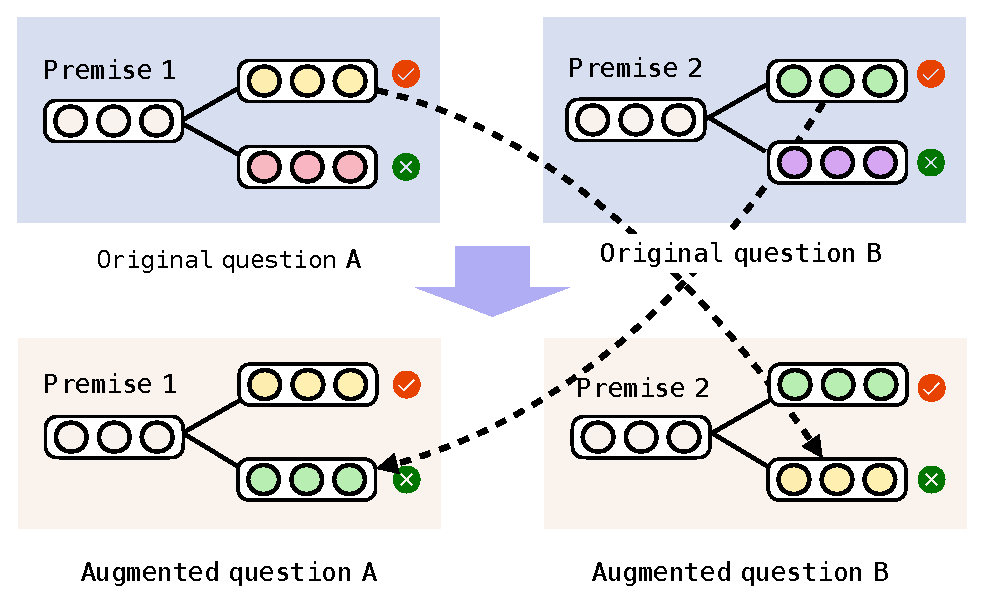
\includegraphics[width=0.85\columnwidth]{figure/aug.eps}
        \caption{Crossover: the rights choice of both questions
                are used to replace the wrong choices of these questions to create
                two new questions. Circles symbolize tokens in the sentences.
		%\KZ{Change the labels of the questions to ``Original question A'',
		%``Original question B'', ``Augmented question A''', etc. Just like
%in the mutation figure. Remove ``Original questions'' and ``Augmented questions''.}
        } 
        \label{fig:cross}
\end{figure}
%Besides the quantity, crossover is a good option for data augmentation,

%If we swapped the wrong choices, we could 
%still produce two legitimate new questions. But these new questions can't
%test short circuit, because: a) if a model
%short-circuits on the right choice of question B (as in \figref{fig:cross}), 
%swapping the wrong choice of B into question A doesn't make A' a good test, 
%since the model is not sensitive to wrong choice; 
%b) if a model short-circuits on the wrong choice of
%question B, swapping the wrong choice of B into A will make A' 
%easier to solve by the model, so it will 
%still pick the right choice and pass the test.

%We can also teach them to discover semantic and syntax problems with the advantage of the choice question format. 
%\KZ{Crossover not only can be used to test for
%short circuit, it can also be used to improve the model
%robustness. How to?}
%Both methods actually have the potential to teach the model 
%to consider the previous premise. First of all,  crossover is a replacement for the ``True'' choices, 
%models can not get the correct answer from the choices alone. 
%\KZ{The crossver operation inspired us to try mutation.}

\subsubsection{Mutation}
\label{sec:mutate}

\textit{Mutation} is illustrated in \figref{fig:mutation}. 
%Similar to \textit{crossover}, 
%\KZ{Always say ``similar to''; there's no such thing as
%``similar with''.} 
%we always preserve the 
%right choice and augment data by changing the wrong choice. 
%\textit{Mutation} 
It is also designed to teach models 
to pay more attention to the relationship between the premise and the choices. 
Different from \textit{crossover} which makes the choices very different, 
\textit{mutation} makes the two choices of a question very similar except for the 
order of the words. This forces the model to look to the premise to avoid short-circuit problems.
%they can be derived from the right choices or wrong choices. For example, In Figure3, The 
%right choice can be denoted as R, the wrong choice with color pink can be denoted as W. 
%Then the swapped sentence from R and W are R' and W'. R' and W' are both wrong choices because 
%they are grammatically wrong. Then we can randomly choose R' or W' as a wrong choice for the 
%new aumgmented question A'.

We reserve the 
right choice and augment data by changing the wrong choice. 
\textit{Mutation} operation swaps two consecutive words~\footnote{The words are 
tokenized with NLTK.} either in 
the right choice or wrong choice of 
the original MCQ, each with 50\% probability, to make a new wrong choice.
%Compared to crossover,
The \textit{mutation} operator should not be confused with the random token
swapping (RS) operator~\cite{artetxe2017unsupervised,lample2017unsupervised}.
RS seeks to perturb a choice in the question without changing its label,
whereas mutating the right choice (\textit{mutation}) converts it to a wrong choice because the 
perturbed choice is ``less right'' than the original one.
Mutating the wrong choice has a similar effect as RS.
%lots of work mentioned randomly swapping tokens (mutation)
%(Artetxe et al., 2018; Lample et al., 2018; Wei and Zou, 2019; Miao et al., 2020),
%The purpose of RS is to improve models' fault tolerance by perturbing
%the sentence without changing its meaning;
%the purpose of our mutation is to encourage the models to look into the
%premise (thus avoid short-circuits).
%Consequently, the way we construct the data is also different. 
Intuitively, mutation has the potential to reduce short circuits:
it not only encourages the model to look into the premise due to its
two very similar choices (see the two choices of A1 in \figref{fig:mutation}),
but also makes the model more sensitive to the differences in word orders 
and enhances the model's pre-existing grammatical knowledge (see the two choices in
A2). 
%Discuss the pros and cons of the two.
%Explain why mutation may not be a good choice for detecting
%short-circuit.
\begin{figure}[th]
        \centering
        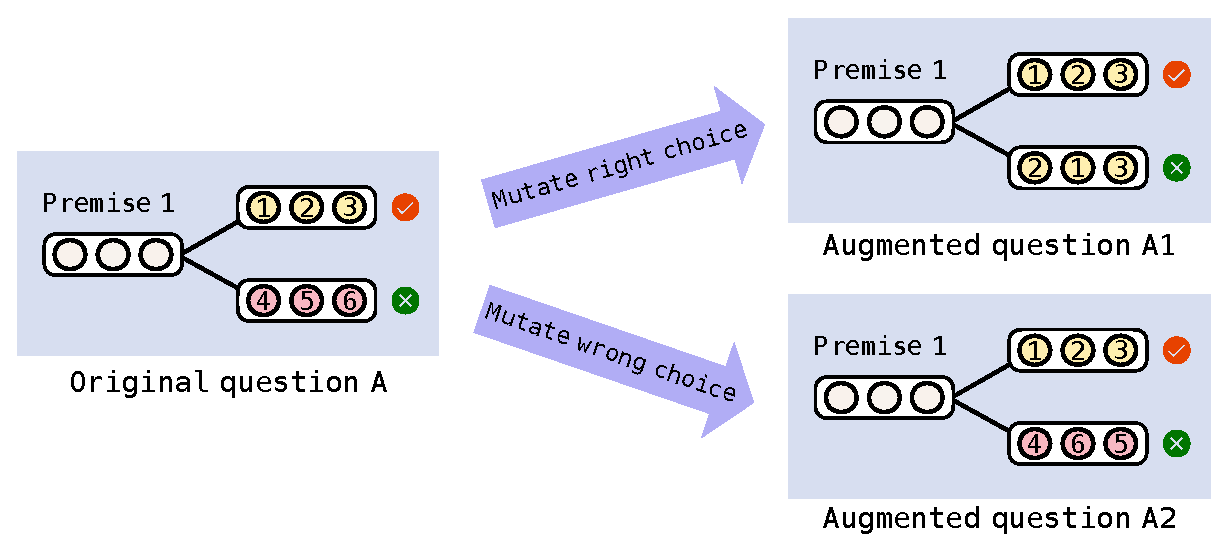
\includegraphics[width=0.9\columnwidth]{figure/revised_mutation.eps}
        \caption{Mutation: the right choice of a question
                is used to replace the wrong choices of this question to create
                new questions. Circles symbolizes tokens.}
        \label{fig:mutation}
\end{figure}



